\section{Check of the background in sideband region}
\label{app:bkg_check}

In the comparison between data and cocktail MC in the $\mbc$ sideband region, discrepancy is observed in the distribution of $M^2(K^-\pi^+)$, as shown in Figure~\ref{fig:comp_datamc_sideband}.
A peaking structure is observed around 0.8 $\gev$ region, which is not described by the cocktail MC samples. There are two kinds of background processes in the cocktail MC samples, including the non-signal $\lcp\lcm$ pair production and inclusive hadron processes. The stack distribution of $M^2(K^-\pi^+)$ of cocktail MC samples is shown in the left of Figure~\ref{fig:bkg_cocktail} at $\sqrt{s} = 4.682\gev/c^2$. The contribution of non-signal $\lcp\lcm$ processes is very small comparing to the hadron one. From the truth information shown in the right of Figure~\ref{fig:bkg_cocktail}, the main process in the selected non-signal $\lcp\lcm$ events is $\lcp \to p K^-\pi^+\pi^0, \lcm \to \bar{\Sigma}^-\pi^-\pi^+$. It could have intermediate resonance of $\bar{K}^*(892)$, but the statistics are too small to describe the structures in data.

\begin{figure}[h]\centering
    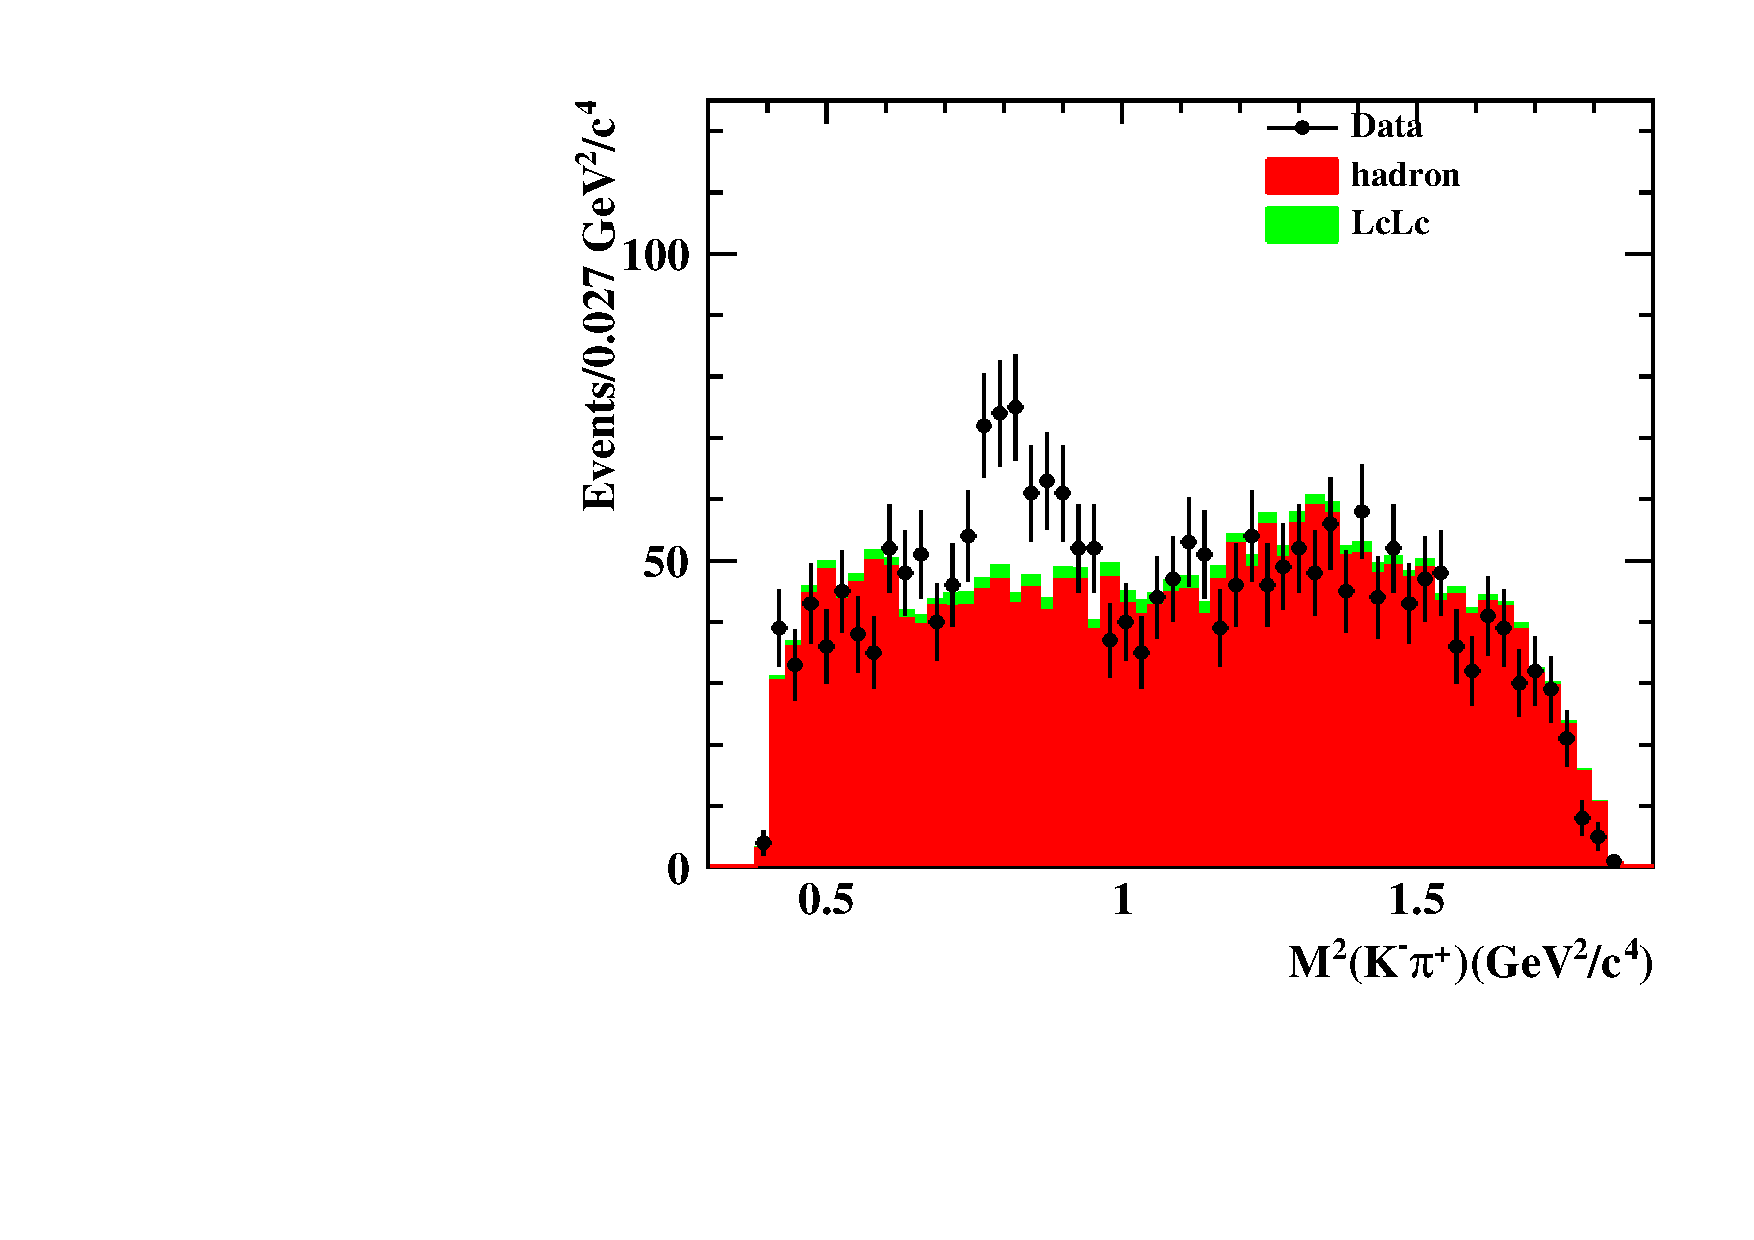
\includegraphics[width=0.45\textwidth]{figure/app_bkg/output_mc_0_sideband_stack_m2_23_2c_1.pdf}
    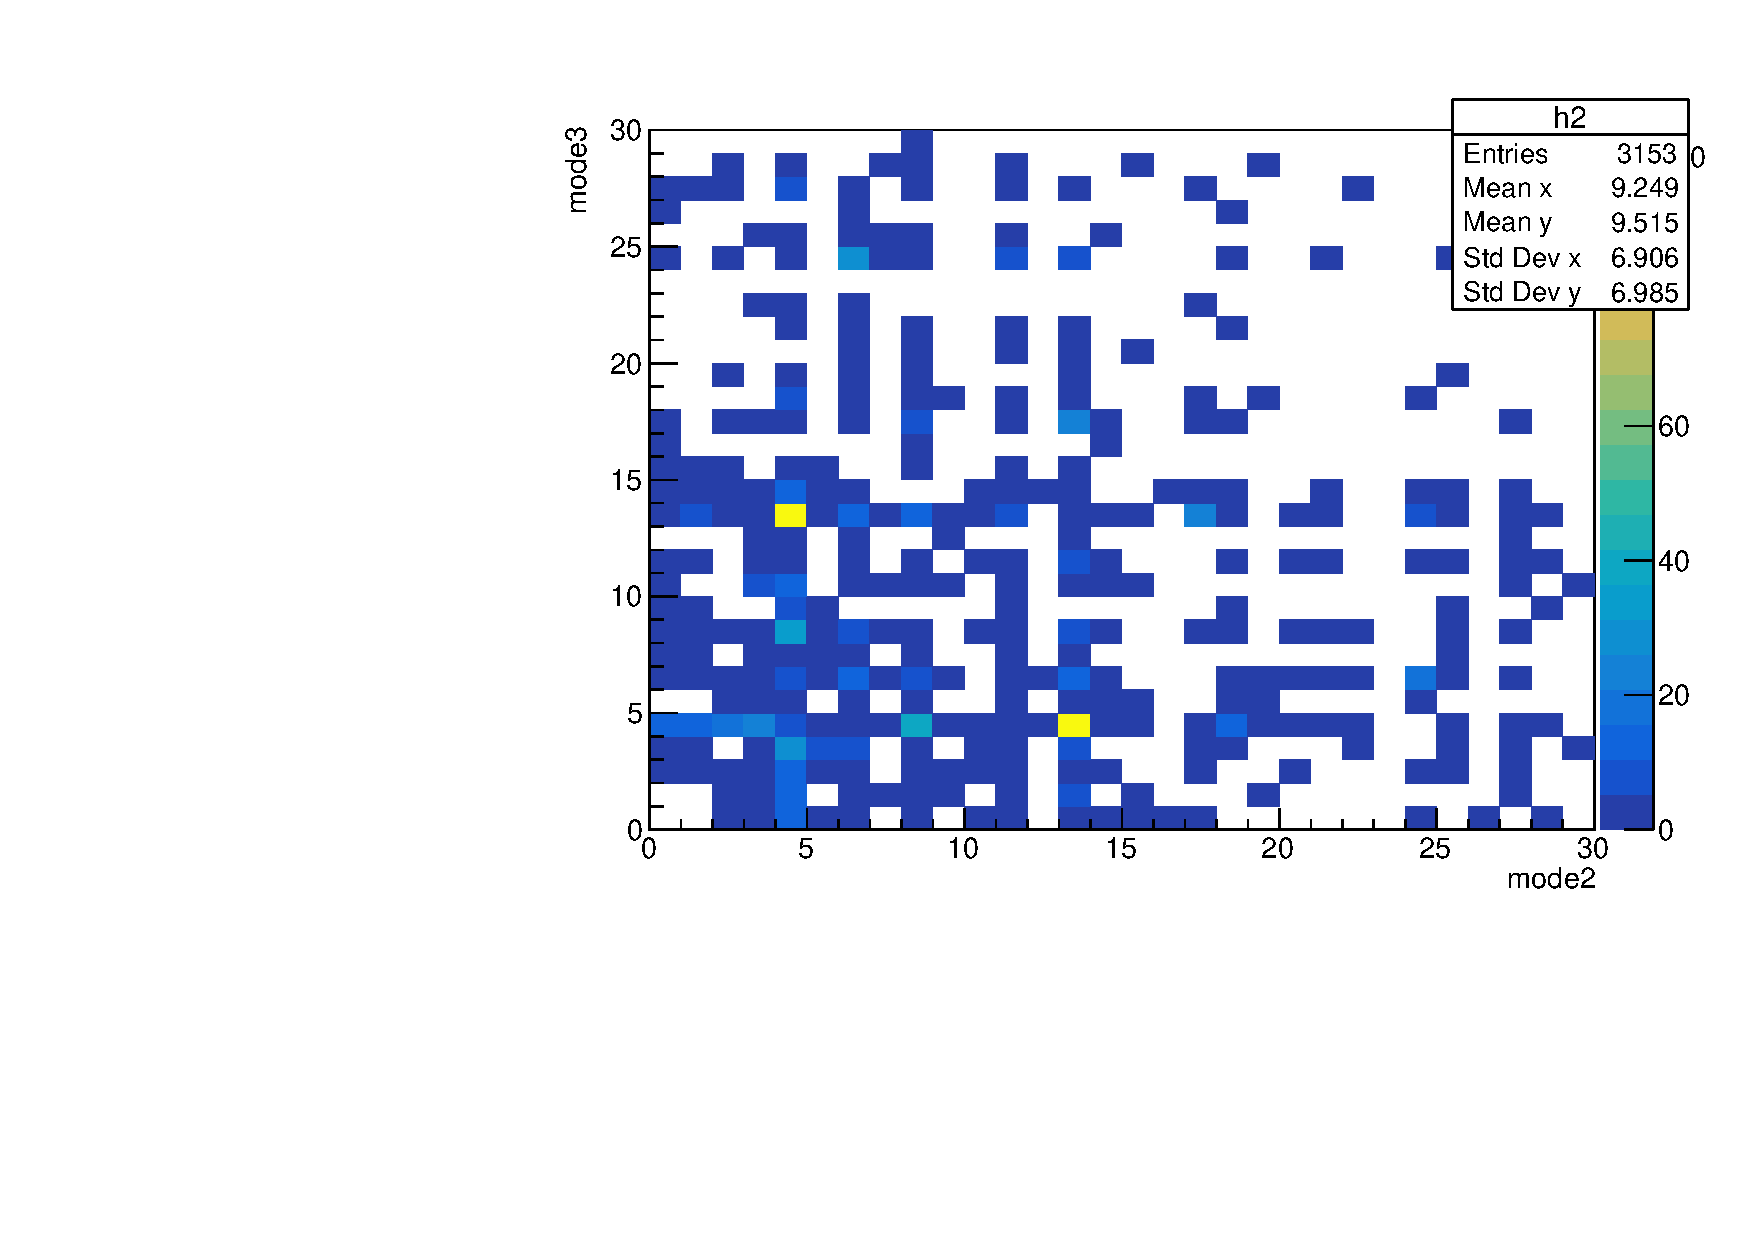
\includegraphics[width=0.45\textwidth]{figure/app_bkg/lclc_bkg_mode.pdf}
    \caption{Stack distribution of $M^2(K^-\pi^+)$ for cocktail MC samples at $\sqrt{s} = 4.682\gev/c^2$ (left). The index of decay channel of $\lcp$ and $\lcm$ in the selected non-signal $\lcp\lcm$ pair MC samples.}
\label{fig:bkg_cocktail} 
\end{figure}

For the hadron samples, a topology analysis is performed with all selection criteria documented in Section~\ref{sec:selections}. An additional cut is applied on the $M(K^-\pi^+)$ distribution within [0.8, 1.0] $\gev/c^2$. The top 21 processes are listed in Figure~\ref{fig:topo_hadron}. The main background source is the mis-identification between Kaon and Pion. The corresponding $\mbc$ distribution of selected hadron events are shown in Figure~\ref{fig:mbc_hadron}. No peaking background is observed in the $\mbc$ signal region.

\begin{figure}[h]\centering
    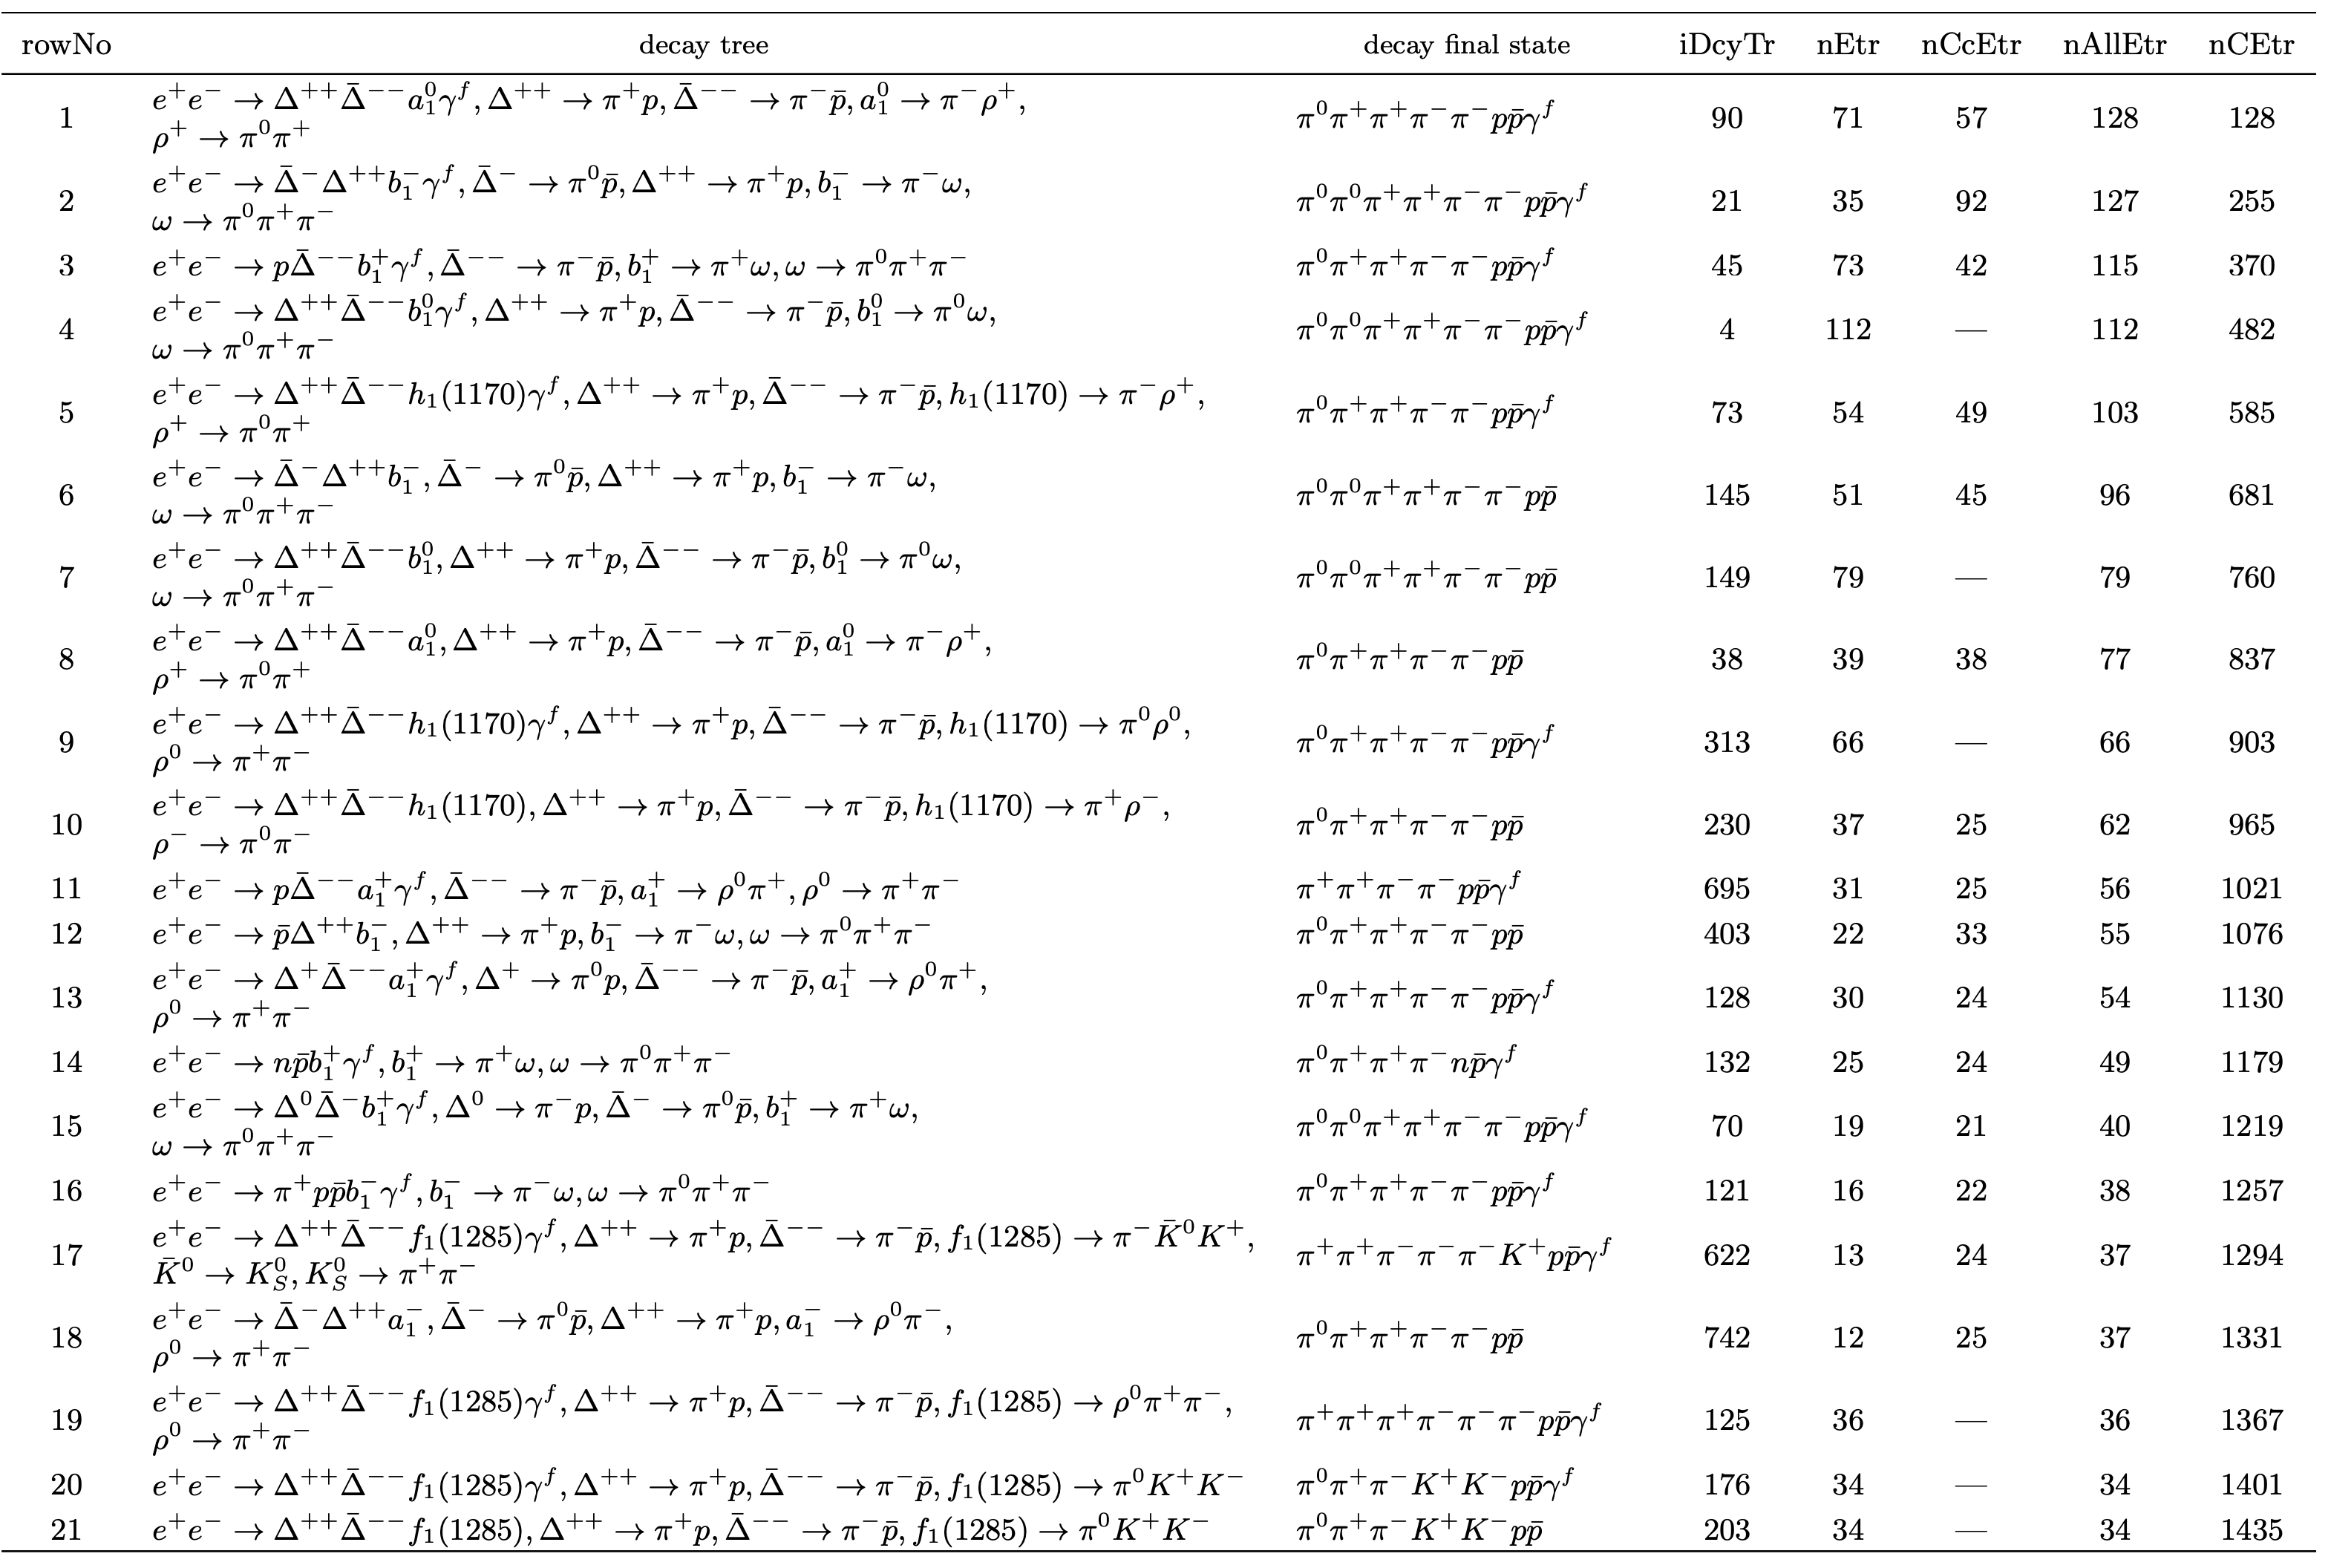
\includegraphics[width=0.90\textwidth]{figure/app_bkg/topo.png}
    \caption{Decay trees and their respective final states in hadron samples.}
\label{fig:topo_hadron} 
\end{figure}

\begin{figure}[h]\centering
    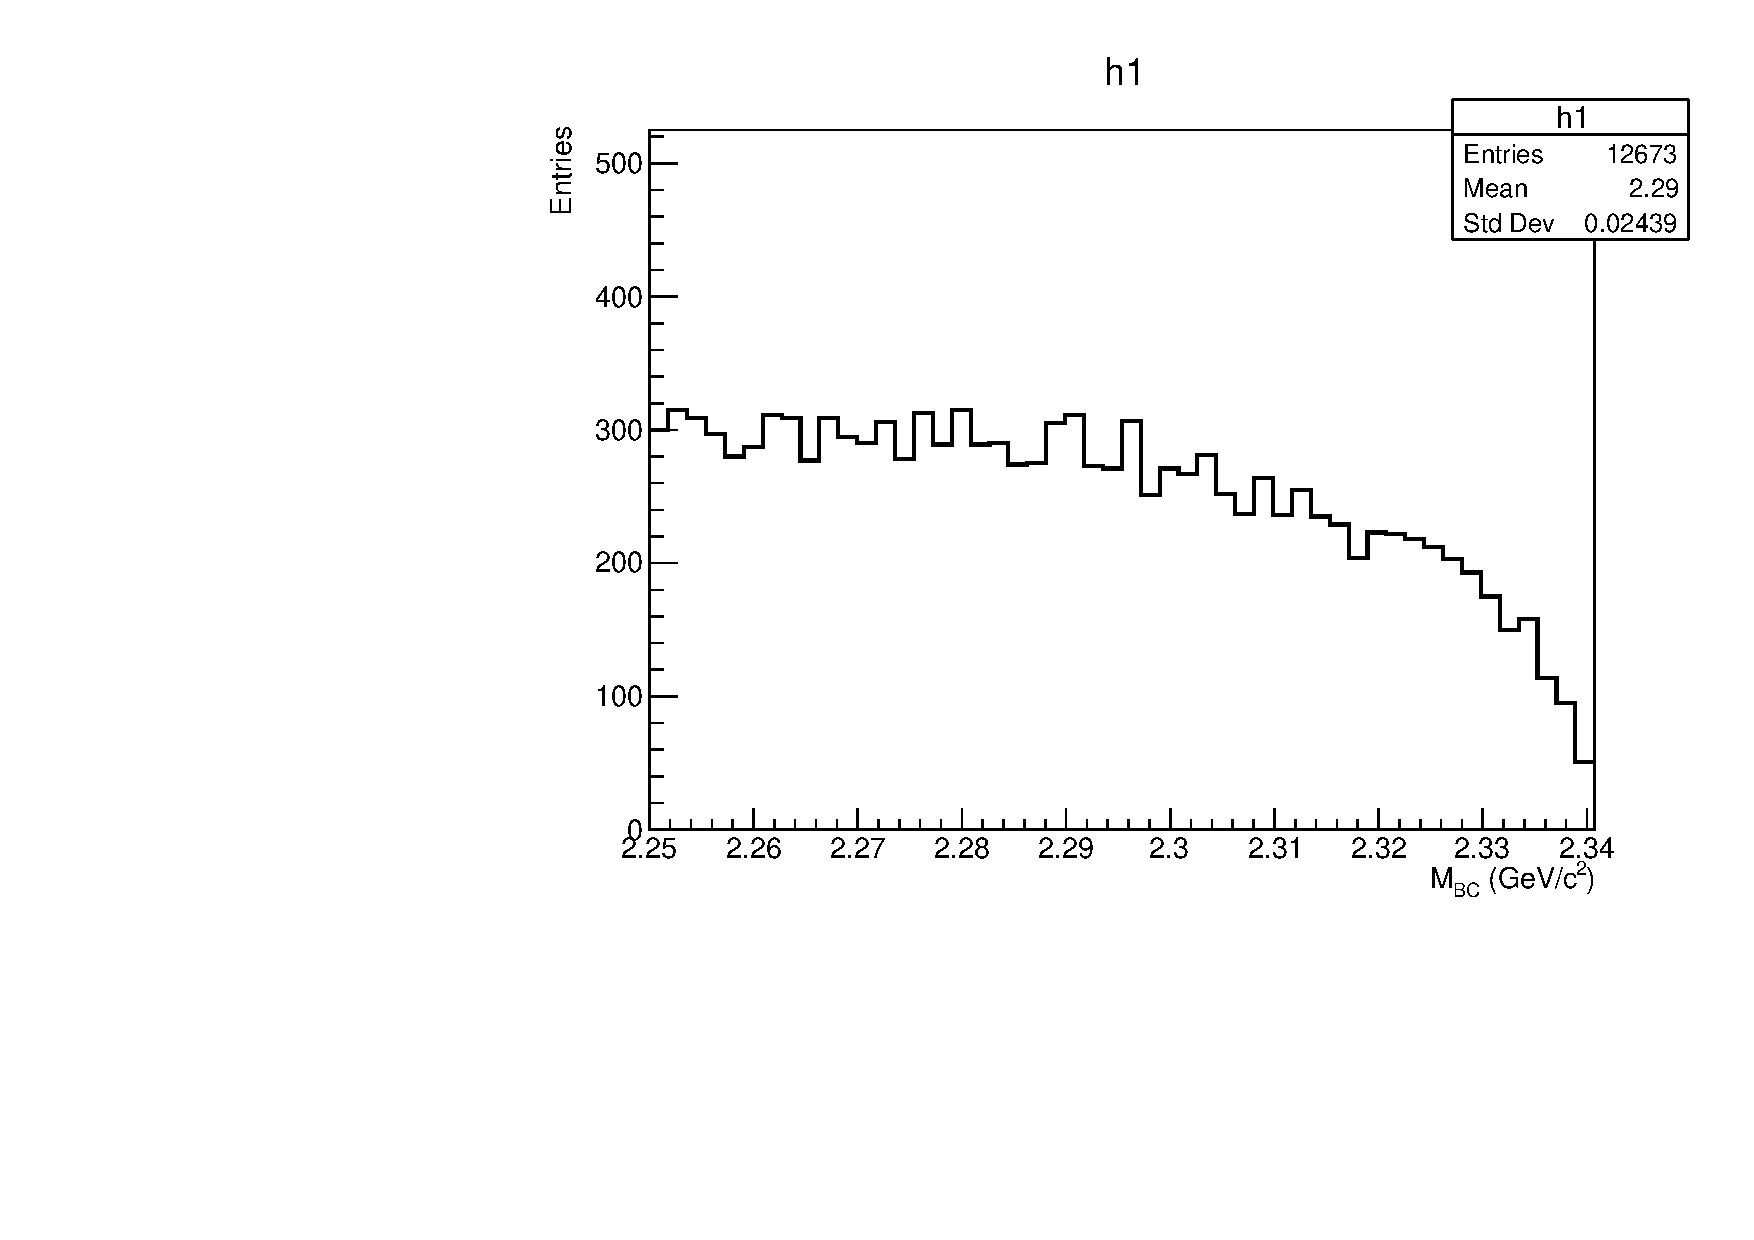
\includegraphics[width=0.60\textwidth]{figure/app_bkg/mbc_hadron.pdf}
    \caption{Distribution of $\mbc$ of hadron samples within [0.8, 1.0] $\gev/c^2$ of $M(K^-\pi^+)$.}
\label{fig:mbc_hadron} 
\end{figure}